\documentclass{article}
\usepackage{fancyhdr}
\usepackage{titlesec}
\usepackage{graphicx}
\graphicspath{ {./img/} }
\usepackage{multirow}
\usepackage[a4paper, total={6in, 8in}]{geometry} % use this package in all paper
\usepackage{hyperref}
\hypersetup{
    colorlinks=true,
    linkcolor=blue,
    filecolor=magenta,      
    urlcolor=cyan,
    pdftitle={Overleaf Example},
    pdfpagemode=FullScreen,
} 

\pagestyle{fancy}
\fancyhf{}
\lhead{Modul 9 Praktikum Jaringan Komputer}
\rfoot{\footnotesize Page \thepage}
\lfoot{\footnotesize Mahyus Ihsan, S.Si, M.Si \newline Jurusan Informatika Universitas Syiah Kuala \newline Modul oleh : Diky Wahyudi, Furqan Al Ghifari, Rendika Rahmaturrizki}
\renewcommand{\headrulewidth}{1pt}
\renewcommand{\footrulewidth}{1pt}

\titleformat*{\section}{\small\bfseries}

\begin{document}
    \begin{center}
        \textbf{Modul 9 Praktikum Jaringan Komputer}

        \textbf{MikroTik}
    \end{center}

    \section*{Deskripsi Singkat}
    \hspace{\parindent} Mikrotik merupakan sistem operasi berupa perangkat lunak yang 
    digunakan untuk menjadikan komputer menjadi router jaringan. 
    Sistem operasi ini sangat cocok untuk keperluan administrasi 
    jaringan komputer, misalnya untuk membangun sistem jaringan komputer 
    skala kecil maupun besar.\\

    MikroTik RouterOS dapat di install pada komputer maupun laptop serta 
    dapat juga diinstall di virtual machine seperti VirtualBox. 
    Untuk menginstall MikroTik RouterOS diperlukan file ISO yang dapat diperoleh 
    melaui situs mikrotik.com. Sistem operasi MikroTik ini hanya bersifat 
    trial dengan durasi waktu 24 jam. Untuk versi penuhnya (full version) 
    dapat dilakukan dengan cara membeli lisensi dari penyedia MikroTik RouterOS. 
    Pada kesempatan kali ini, kita akan mencoba menyajikan panduan instalasi 
    MikroTik di VirtualBox.


    \section*{Tujuan}
    \begin{enumerate}
        \item Mengetahui fungsi-fungsi MikroTik 
        \item Mampu melakukan instalasi MikroTik Router OS di virtualbox 
        \item Mampu melakukan konfigurasi dasar MikroTik di virtualbox
        \newline 
    \end{enumerate}


    % theory section

    \begin{flushleft}
        \textbf{Materi 1 - Instalasi Mikrotik RouterOS di VirtualBox}

        pertama kali, kita akan mendownload \textbf{virtualbox} dan \textbf{mikrotik os} terlebih dahulu \\
        
        \begin{itemize}

        	
			\item \textbf{Download Virtualbox} \\
				Silahkan kunjungi link berikut untuk mendownload \href{https://www.virtualbox.org/}{virtualbox}. Pilih sesuai dengan OS yang digunakan. Jika menggunakan Windows, maka pilih \textbf{Windows hosts} \\
				
				\begin{center}
					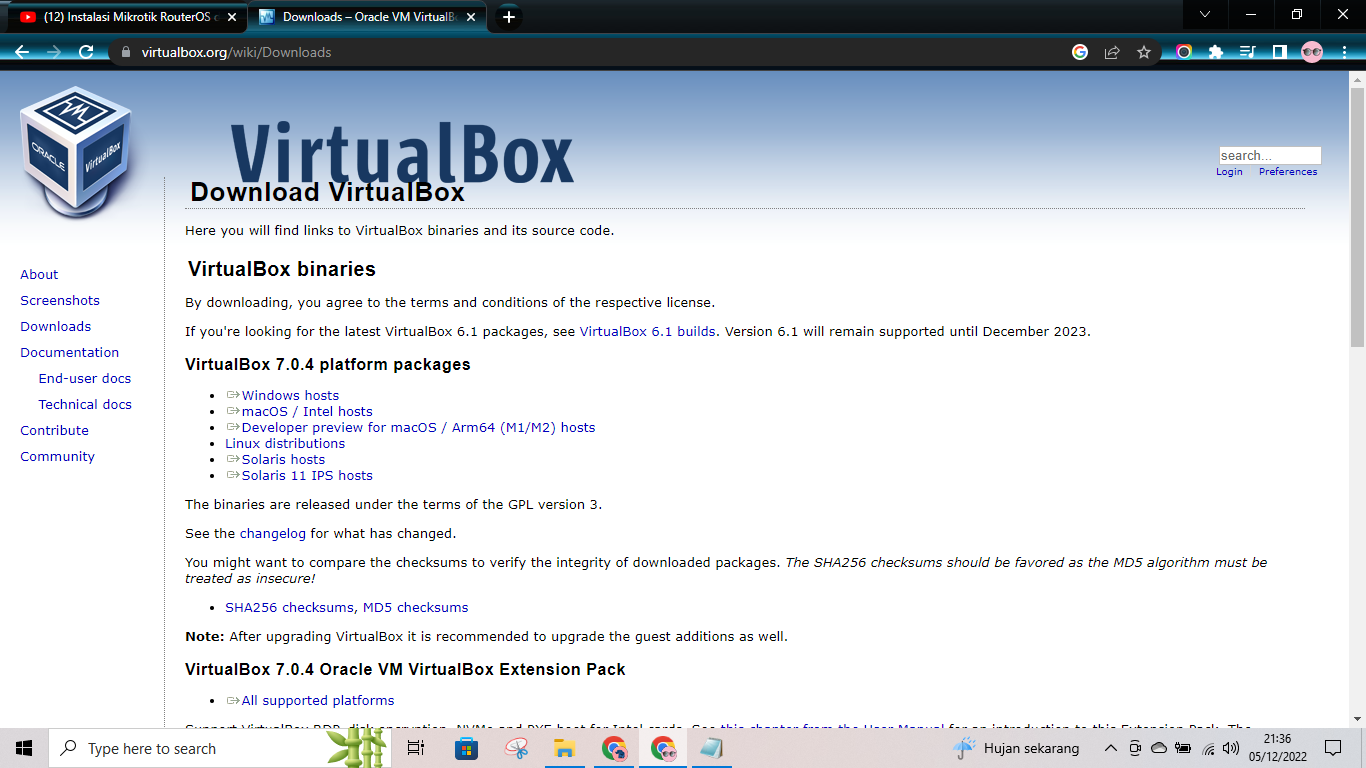
\includegraphics[scale=0.3]{Screenshot1} \\
					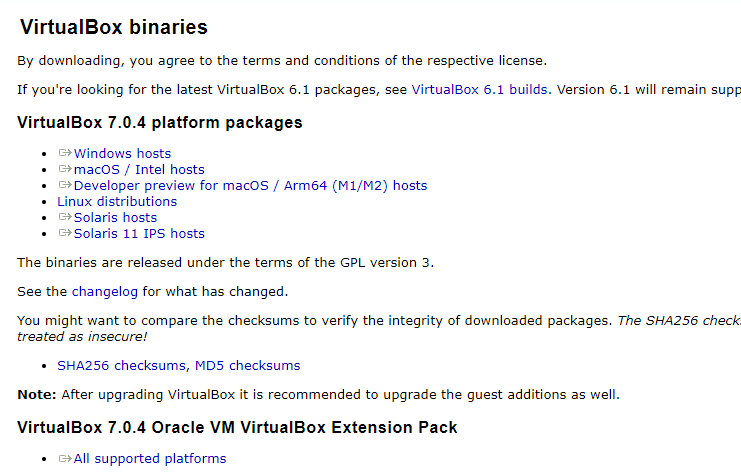
\includegraphics[scale=0.4]{Screenshot1.2} \\       	
        		\end{center}
				
				Klik dua kali file \textbf{VirtualBox} yang telah diinstal, lalu klik \textbf{Next}
				
				\begin{center}
					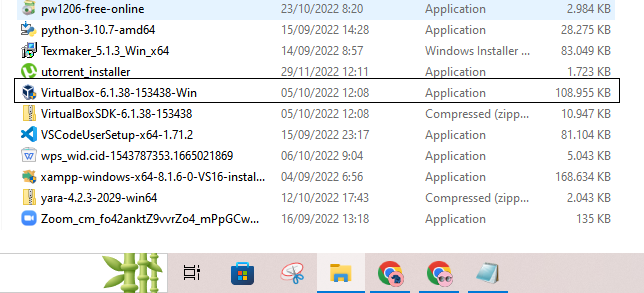
\includegraphics[scale=0.6]{Capture2.1} \\~\\
					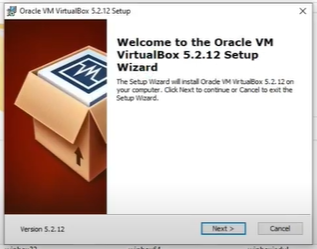
\includegraphics[scale=0.8]{Capture} \\       	
        		\end{center}
        		
        		Klik \textbf{Next \>}
        		
        		\begin{center}
        			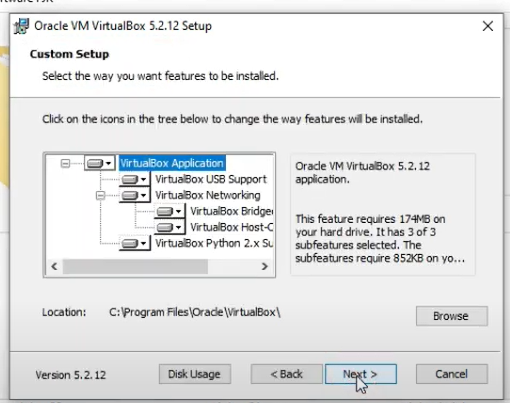
\includegraphics[scale=0.7]{Screenshot (253)} \\
        		\end{center}
        		
        		Pastikan semuanya tercentang, kemudian klik \textbf{Next \>} \\
        		
        		\begin{center}
        			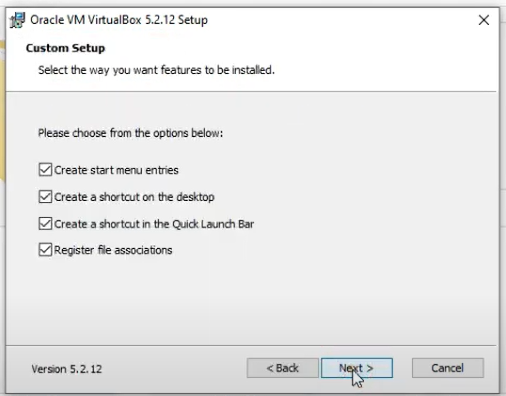
\includegraphics[scale=0.7]{Screenshot (254)} \\
        		\end{center}
        		
        		Klik \textbf{Yes}
        		
        		\begin{center}
        			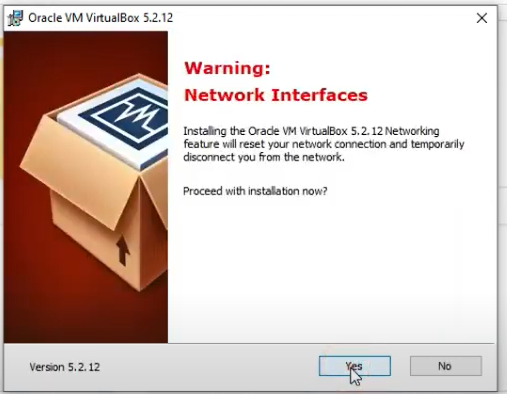
\includegraphics[scale=0.7]{Screenshot (255)} \\
        		\end{center}
        		
        		Kemudian klik \textbf{Install}. Tunggu hingga proses instalasi selesai, kemudian klik \textbf{Finish}
        		
        		\begin{center}
        			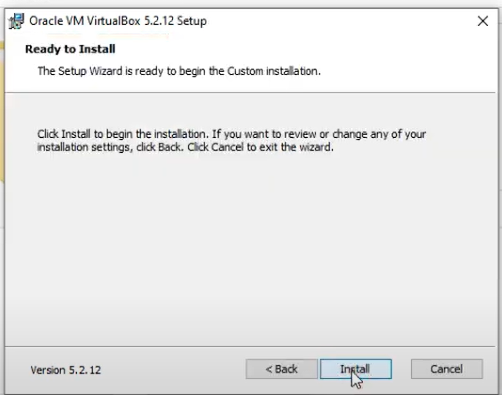
\includegraphics[scale=0.7]{Screenshot (256)} \\~\\
        			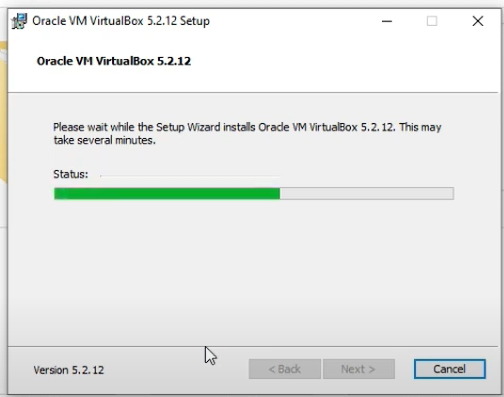
\includegraphics[scale=0.7]{Screenshot (257)} \\~\\
        			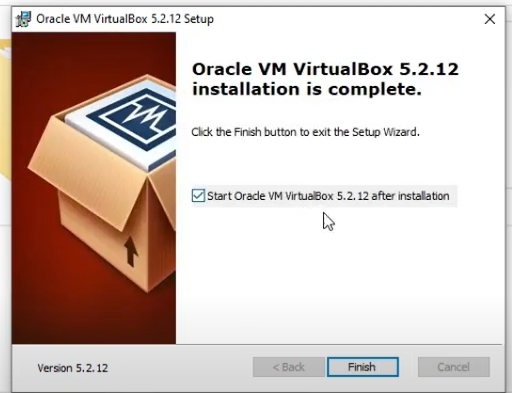
\includegraphics[scale=0.7]{Screenshot (258)} \\
        		\end{center}
        		
				Jika tidak ada kesalahan pada saat penginstalan, tampilan \textbf{virtualbox} seperti dibawah ini akan muncul
        		
        		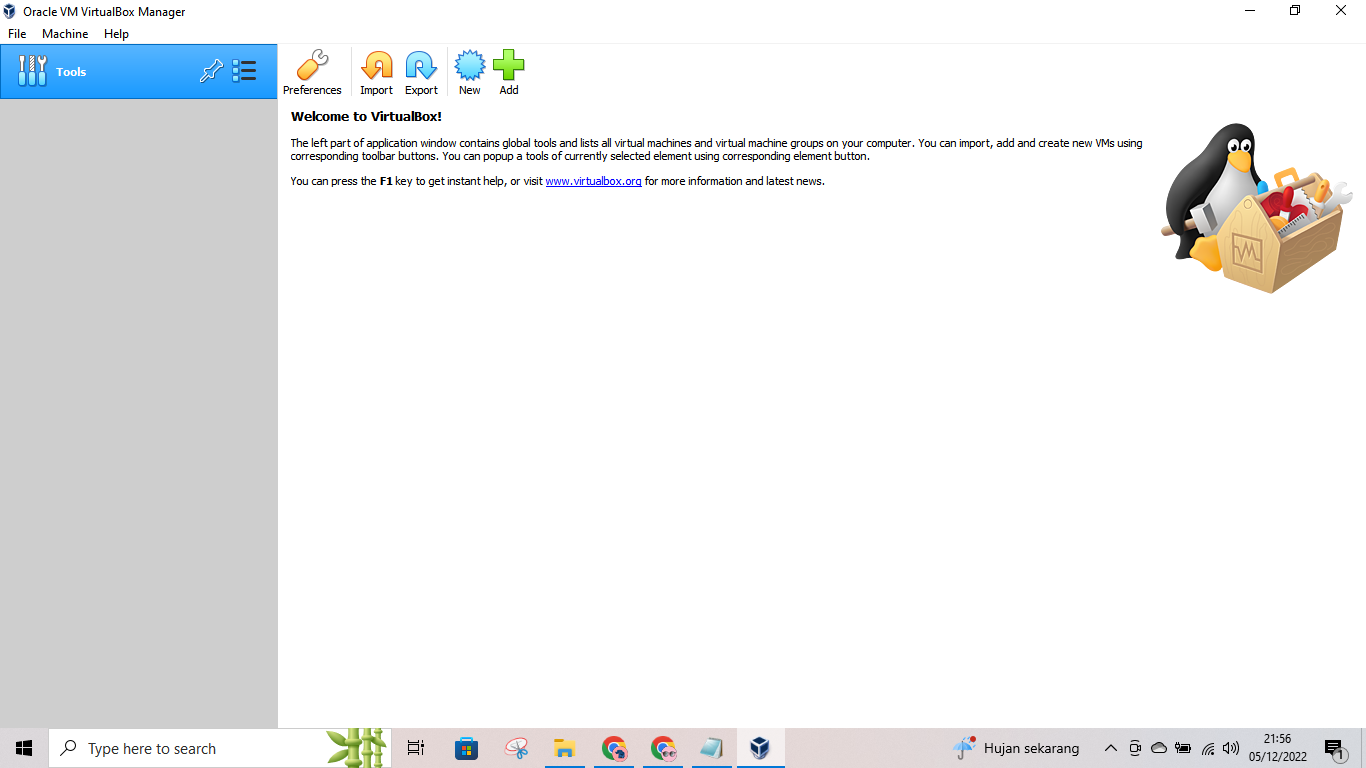
\includegraphics[scale=0.3]{vbox} \\~\\ 
        	
			\item \textbf{Download Mikrotik OS} \\
				Silahkan kunjungi link berikut untuk mendownload \href{https://mikrotik.com/download}{Mikrotik Router OS}. Klik \textbf{RouterOS v6} 
				
				\begin{center}
					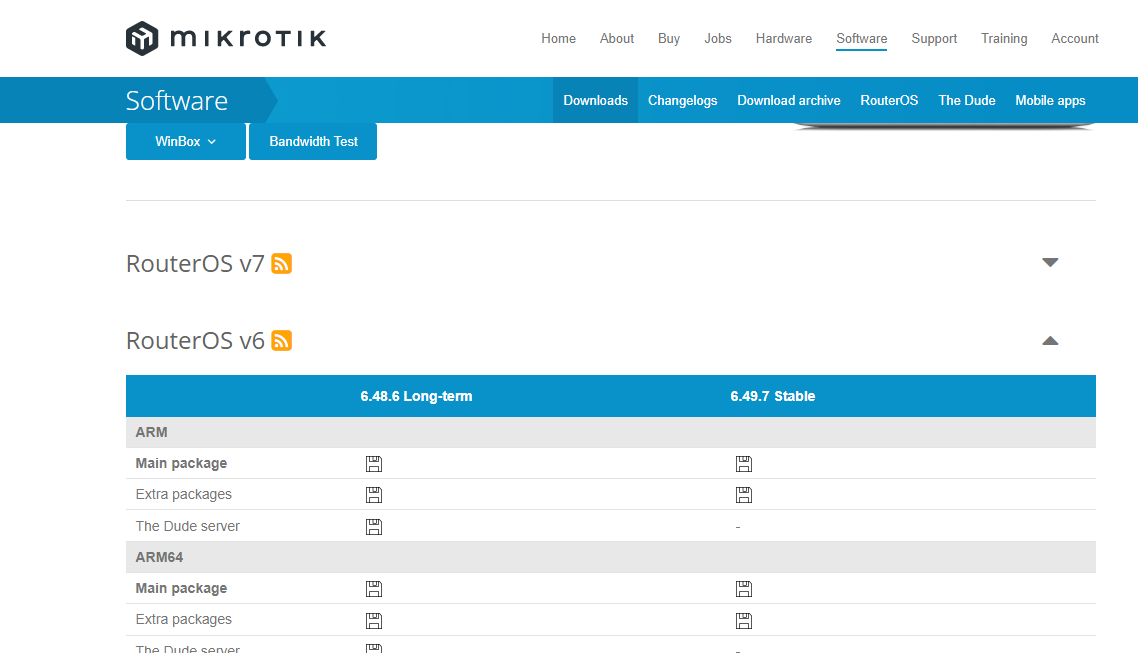
\includegraphics[scale=0.3]{routerOS} \\
				\end{center}
				
				Scroll ke bawah sampai menemukan untuk pilihan \textbf{x86}. Klik \textbf{CD image} versi stable (yang sebelah kanan). Mikrotik OS akan otomatis terinstall
				\begin{center}
					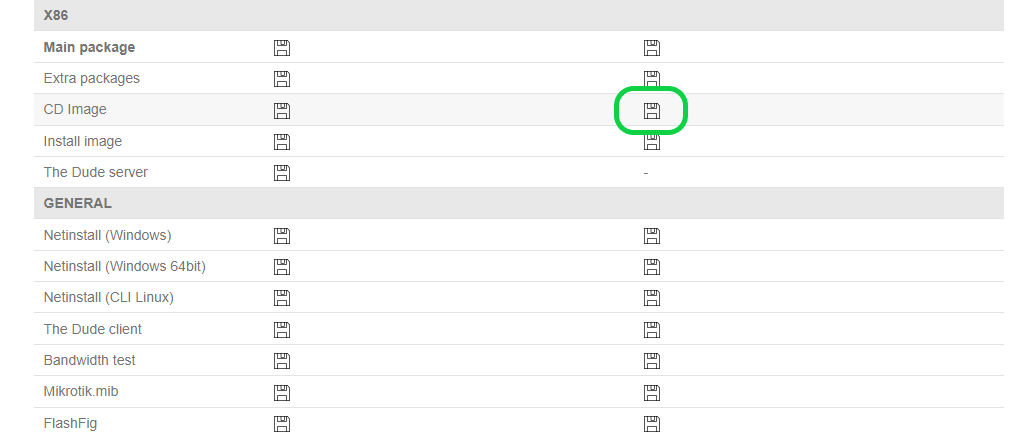
\includegraphics[scale=0.3]{routerOS2} \\
				\end{center}				 
 				        	
        	
        \end{itemize}

    \end{flushleft}

	\newpage
    \begin{flushleft}
        \textbf{Materi 2 - Konfigurasi MikroTik pada VirtualBox}
        \newline

        sebelum melakukan konfigurasi mikrotik, persiapkan mikrotik dengan melakukan instalasi di virtualbox \\
        
        \begin{itemize}
        	
        	\item Klik \textbf{New} \\
        		\begin{center}
        			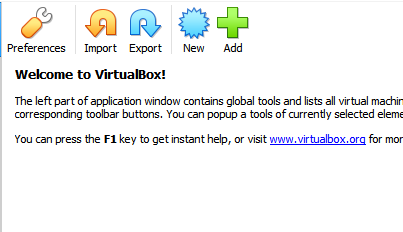
\includegraphics[scale=0.6]{virtualbox}
        		\end{center}
        		
        	\item Berikan \textbf{Name:} sesuai dengan yang kalian inginkan, atur \textbf{Type:} dan \textbf{Version:} sesuai dengan gambar dibawah\\
        		\begin{center}
        			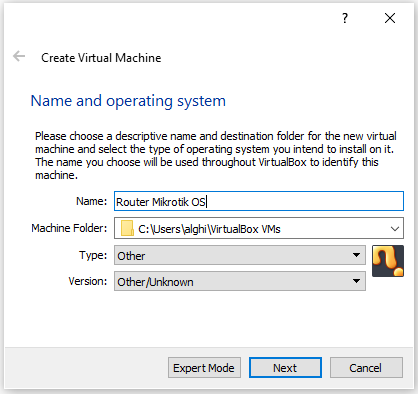
\includegraphics[scale=0.6]{(2)}
        		\end{center}
        	
        	\item Berikan ukuran \textbf{Memory size:} sebesar \textbf{64 MB} \\
        		\begin{center}
        			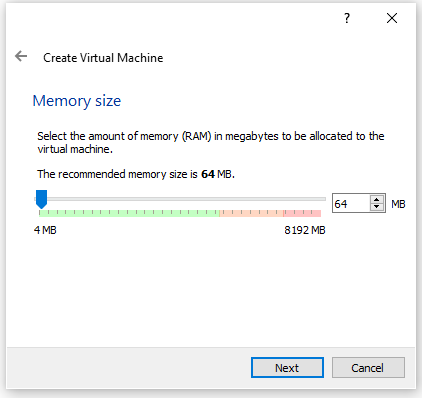
\includegraphics[scale=0.6]{(3)}
				\end{center}
				
			\item Sesuaikan seperti pada gambar dibawah \\
        		\begin{center}
        			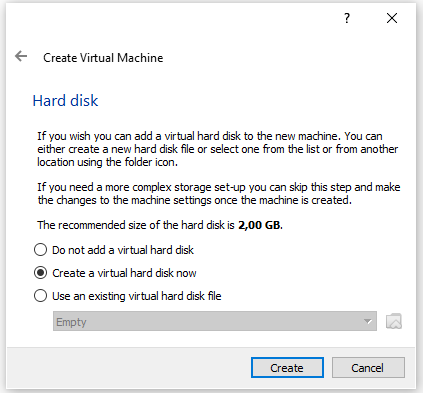
\includegraphics[scale=0.6]{(4)} \\
        			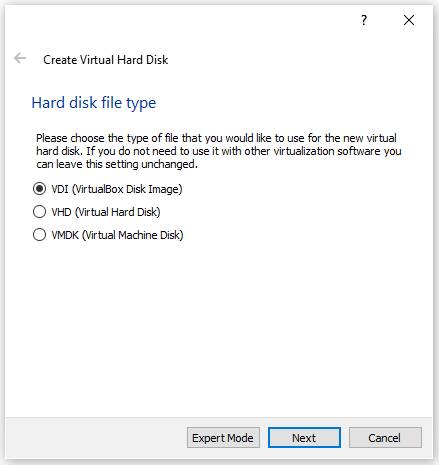
\includegraphics[scale=0.6]{(5)} \\  
        			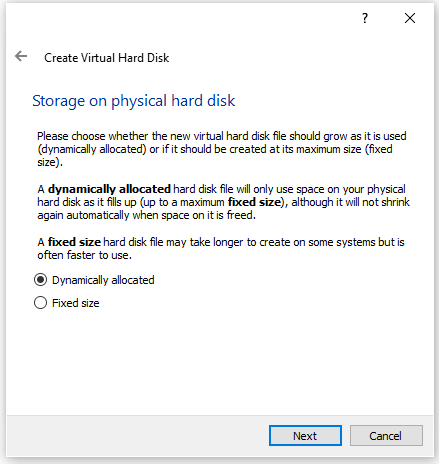
\includegraphics[scale=0.6]{(6)} \\
        		\end{center}
        		
        	\newpage
        	\item Berikan ukuran penyimpanan sebesar \textbf{2,00 GB} \\
        		\begin{center}
        			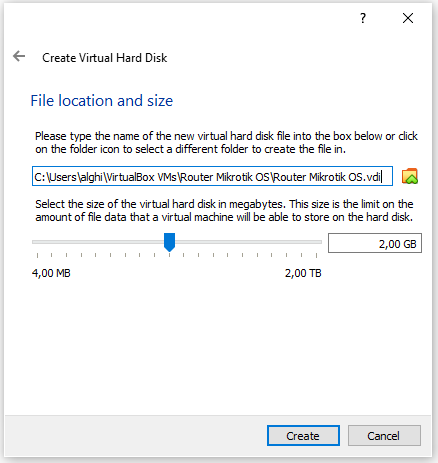
\includegraphics[scale=0.6]{(7)}
        		\end{center}
        	
        	\item Jika tidak ada error, maka akan muncul tampilan seperti dibawah \\
        		\begin{center}
        			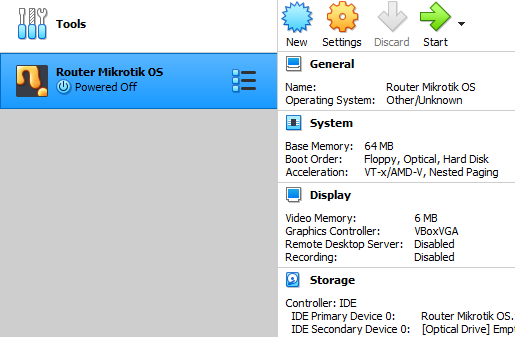
\includegraphics[scale=0.6]{terakhir}
        		\end{center}
        		        	 
        \end{itemize}
        
        Jika sudah menginstall mikrotik OS nya, langkah selanjutnya adalah melakukan beberapa settingan untuk virtual machinenya
        
        \begin{itemize}
        	
			\item pastikan virtual machine yang dibuat sudah terpilih (berwarna biru), kemudian klik \textbf{Settings} 
				\begin{center}
					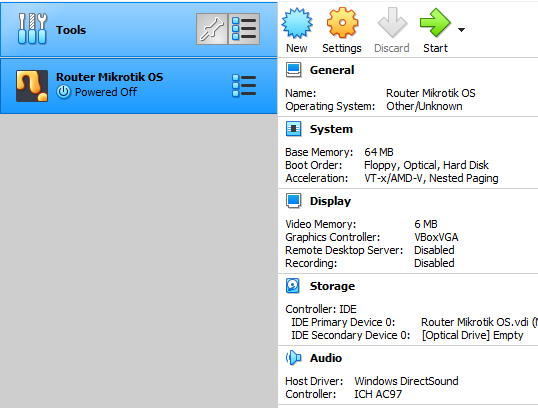
\includegraphics[scale=0.6]{(a)} 
				\end{center}
				
			\item pilih menu \textbf{Storage}, klik tulisan \textbf{Empty}, pilih menu \textbf{Choose a disk file}
				\begin{center}
					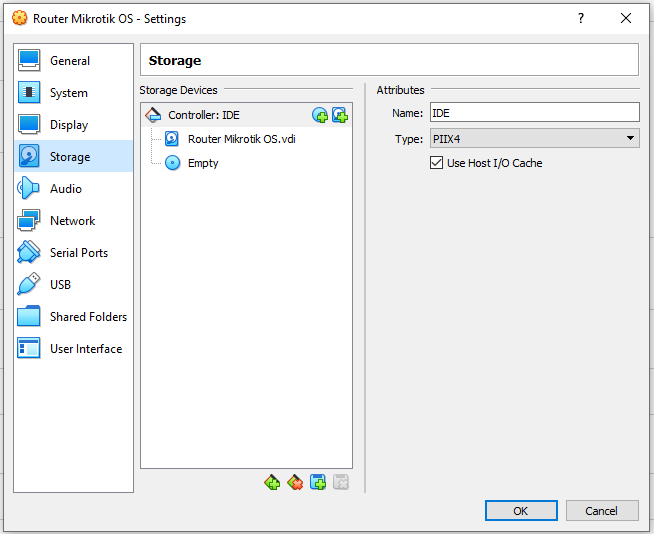
\includegraphics[scale=0.6]{(b)} \\
					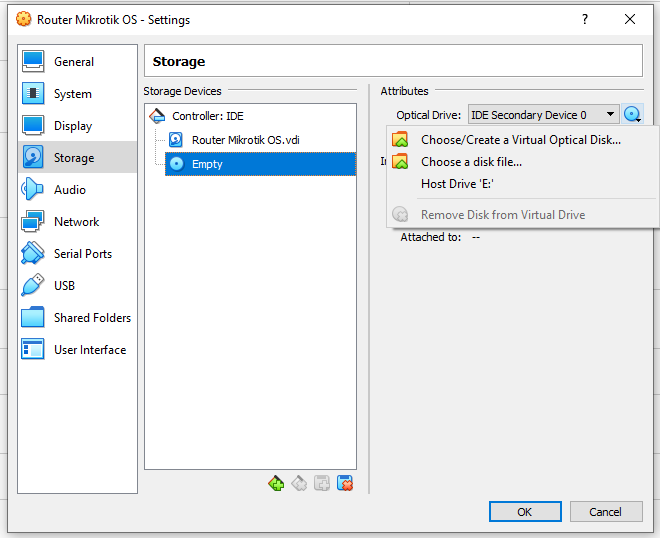
\includegraphics[scale=0.6]{(c)} 
				\end{center}
				
			\item pilih file \textbf{.iso} yang diinstall sebelumnya, kemudian klik \textbf{Open}
				\begin{center}
					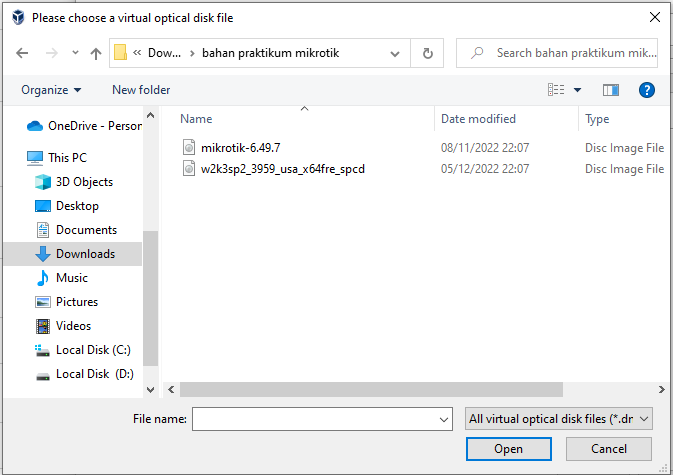
\includegraphics[scale=0.6]{(d)} 
				\end{center}
				
			\item jika sudah, maka muncul seperti dibawah 
				\begin{center}
					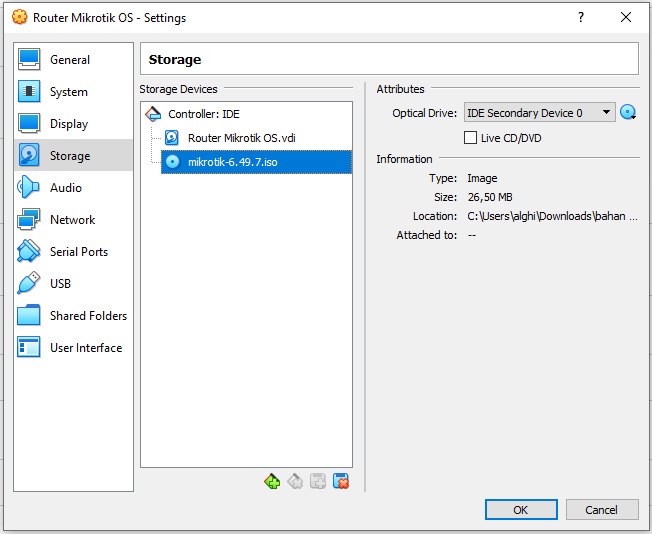
\includegraphics[scale=0.6]{(c.1)}
				\end{center}
			
			\item kemudian kita akan berpindah ke menu \textbf{System}. klik \textbf{Hard Disk} pada pilihan \textbf{Boot Order:}, klik tanda panah ke atas sampai \textbf{Hard Disk} mencapai posisi paling atas 
				\begin{center}
					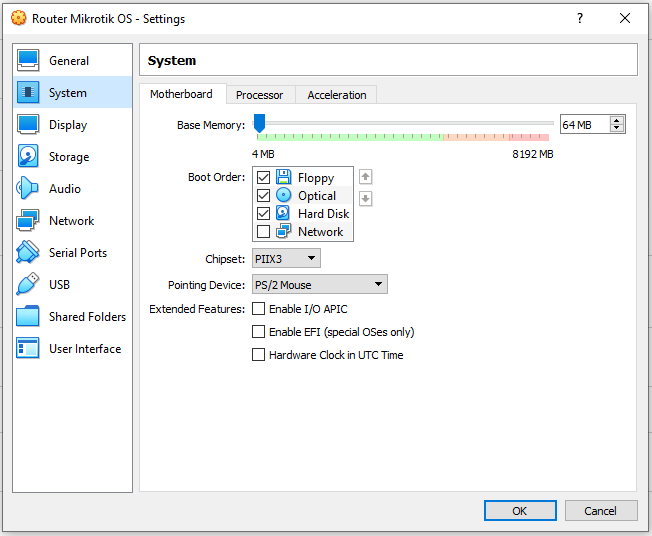
\includegraphics[scale=0.6]{(e)}
				\end{center}
			
			\item nanti akan menghasilkan hasil seperti pada gambar dibawah 
				\begin{center}
					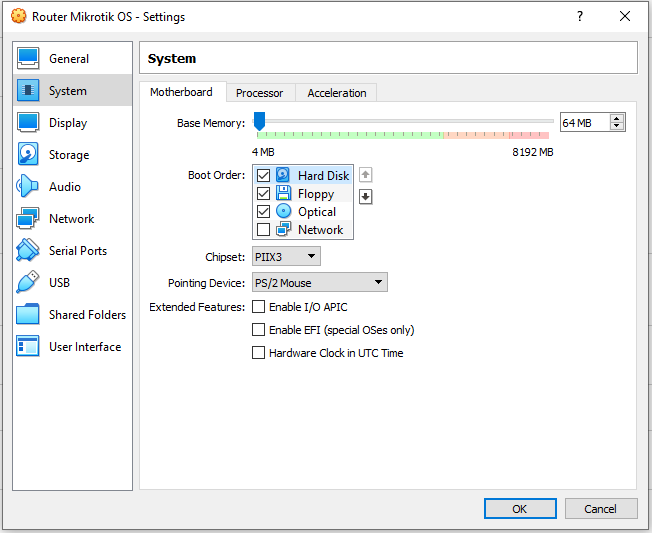
\includegraphics[scale=0.6]{(e)true}
				\end{center}
						
			\item setelah itu, klik tombol \textbf{Ok}
					        	
        	
        \end{itemize}
		
    \end{flushleft}

    \begin{flushleft}
        \textbf{Bonus - Mempelajari fitur fitur yang dapat dilakukan menggunakan MikroTik}
        \newline

        Untuk materi lebih lanjut terkait dengan pembelajaran MikroTik, silahkan kunjungi website 
        \href{https://www.youtube.com/playlist?list=PLvT7-AKYOYMxXuwYv1uA9e0aDsX1XgF4l}{Seri Belajar Mikrotik}\\

        \begin{center}
            \footnotesize\textbf{* Note :} Jika anda belum memiliki device MikroTik, anda dapat 
            menggunakan VirtualBox sebagai sarana pembelajaran simulasi\\
        \end{center}

    \end{flushleft}


    % practice section
%     \newpage
%     \begin{flushleft}
%         \textbf{Tugas}
%         \newline

%         \begin{enumerate}
%             \item Tugas 1
%             \item Tugas 2
%         \end{enumerate}
%     \end{flushleft}

 \end{document}

